\documentclass[12pt, letterpaper, openany]{book}
	\usepackage{graphicx}
	\usepackage{natbib}
	\usepackage[margin=1in]{geometry}
	\usepackage{longtable}
	\setlength{\parskip}{1em}
	\usepackage{pdfpages}
	\usepackage{pifont}
	\usepackage{enumitem}
	\usepackage{titlesec}
		\titleformat{\chapter}{\normalfont\huge}{\thechapter.}{20pt}{\huge\bf}
		\titlespacing{\section}{0pt}{*3}{*0}
		\titlespacing{\chapter}{0pt}{*-2}{*3}
		\titlespacing{\subsection}{0pt}{*0}{*0}
		\titlespacing{\subsubsection}{0pt}{*0}{*0}
		\renewcommand{\chaptername}{}
	\usepackage{enumitem}
		\setlist{itemsep=.5pt}

\title{
\includegraphics[scale=0.35]{../../../img/logo.png}\\Applied Rationality Handbook}
\author{Berkeley 2016}
\date{}
\pagestyle{headings}

\begin{document}
	\frontmatter
	\maketitle
	\mainmatter
	\tableofcontents
	\part*{Day 0}
		\addcontentsline{toc}{part}{Day 0}		
		\chapter{What is ``Applied Rationality''?}
				\chapter*{What is ``Applied Rationality''?}
	
	\section*{Aiming to answer the right questions \ldots}
	Imagine that an intelligent, curious person meets with you for lunch, and begins asking you about your field of expertise.  At first, you talk mainly about your own day-to-day work, but eventually the conversation turns to the big, open questions---what are the most important unsolved problems in your profession?  Why do they matter?  What kinds of things change once you and your colleagues break through?  After you share your perspective, your new acquaintance nods thoughtfully, and asks one final question:
	
	``So, why aren't you working directly on \emph{that}?"
	
	There's a useful (and somewhat friendlier) generalization of this way of thinking.  At any given time in our lives, it's possible (though not always easy!) to answer the question, ``What is the \emph{most} important problem here, and what are the things that are keeping me from working on it?"  We refer to this as ``asking the Hamming question," as a nod to mathematician Richard Hamming, who was notorious for doing the above with his colleagues at Bell Laboratories.
	\\
	\section*{\ldots while accounting for cognitive imperfections.}
	When we make decisions and analyze information, we tend to move back and forth between two broad kinds of thought---one faster, more automatic, and more closely tied to our emotions, and the other slower, more effortful, and more closely tied with our explicit thoughts and beliefs.  In his book \emph{Thinking Fast and Slow}, Nobel Prize winner Daniel Kahneman described them as \textbf{System 1} and  \textbf{System 2}:
	
	\renewcommand{\arraystretch}{1.2}
		\begin{table} \small \centering
			\begin{tabular}{ |c|c| }
			\hline
			\textbf{System 1} &  \textbf{System 2} \\
			\hline \hline
			 Evolved earlier & Evolved later, more unique to humans \\
			 Wordless, ``black box'' thinking & Verbal, ``transparent" thinking \\
			 Processes information quickly & Processes information slowly \\
			 ``Intuition,'' ``reflex,'' etc. & ``Concentration,'' ``reflection,'' etc. \\
			 Always on & Often on standby \\
			 Doesn't use working memory & Limited by working memory \\
			 \hline
			 \end{tabular}
		\end{table}
	 
	 Each ``system'' is complex, made up of a variety of parts, and neither is perfect.  Our knee-jerk, automatic processes are prone to making the wrong connections---if a new acquaintance resembles an old enemy, you may find yourself feeling anxious or cold without really knowing why.  Our deliberate, explicit processes can fail by leaving out information---if you can't put a fleeting feeling of unease into words, you may be tempted to disregard it, and exclude it from your calculations.
	 
	 Often, people make the mistake of thinking that rationality is the process of muting those primitive, intuitive processes and just relying on System 2.  It's an understandable mistake---after all, those are the ``higher brain'' functions, the ones that allow us to do things animals can't, like writing and philosophy and math and science.
	 
	 But turning off or ignoring large parts of your brain is rarely helpful, and applied rationality is about using \emph{every} tool in your possession.  In the classes at this workshop, we'll talk about how to balance and combine these two types of thinking, learning to understand the strengths of each so that you know when to bring them to bear and how to use them effectively both together and apart.  The aim is to make deliberate, thoughtful use of your \emph{whole} mind---a whole that's much greater than the sum of its parts.

\begin{center}

\includegraphics[width=\textwidth]{../../../img/lineshalf.png}
\end{center}		
		\chapter{Advice from Opening Session}
			\section*{``Bad poets borrow---good poets \emph{steal}.''}

If you set out to write a poem, you may find that a particular turn of phrase from another poem just won't stop popping into your thoughts.  Somehow, Homer's reference to the sun as \emph{extending rosy fingers} is exactly what you're trying to say, and you're tempted to just drop it in and call it an homage.

\setlength{\parindent}{1.5em}
But a funny thing is likely to happen here if you actually use Homer's quote (especially if you found yourself borrowing from other sources, too).  There's a certain kind of smoothness and cohesion that's going to be missing---an irregularity of style and pacing that makes your poem come across as a collection of fragments instead of a single unified whole.  It might be a \emph{nice} poem, but it won't be as vivid, as \emph{true,} as what you hoped to convey.

By way of contrast, you could steal the \emph{source} of Homer's thinking---give yourself the same input, rather than simply mimicking his output.  Put yourself in Homer's sandals---how did he come to produce that particular illustration of a dawning day?  What way of looking at the world, and of experiencing language, allowed him to come up with that exact expression?  We only get to see Homer's work, not his actual process, but if you try, you can peer behind the words, and get a glimpse of the source that generated them---of a \emph{way of thinking} that you can emulate to create your own original beauty.

In a similar way, applied rationality as it is presented in this book is the output of other minds.  It's a product you can't \emph{quite} steal for yourself---if you try, you'll find that it never quite fits.  The techniques are excellent algorithms for improving thinking and solving problems, but they aren't the heart and soul of rationality, any more than rosy fingers are the essence of Homer's genius.  They're a jumping-off point, and what you want to jump \emph{toward} is the place the techniques came from---the particular way of thinking about the world and about ourselves that led to someone sitting down and inventing the contents of this book.

This is the real goal of your practice.  As you work through the techniques, try to see this underlying essence.  Aim for a combination of openness and hubris---that is, act like a person who has something to learn, but \emph{also} like a person who's already in possession of a lifetime of knowledge and experience.  Assume that you have joint ownership over your own rationality education, and over the subject of applied rationality as a whole.  We find that the people who get the most out of our workshops are the ones who are simultaneously curious and confident---they're the ones who walk away with all of our techniques \emph{and} the ability to create new techniques of their own.



			\clearpage
\section*{Try Things!}

When you're considering adopting new habits or ideas, there's no better way to gather data than \emph{actually trying.}  It's often faster and simpler to just give things a shot and see how it goes than to spend a lot of time trying to anticipate and predict whether or not you'll find something worthwhile.

This is particularly important because when something \emph{does} work out, \emph{you get to keep doing it.}  If your friends have recommended five different activities to you, and you've only liked one of them, it's easy to think of the whole process as a pretty big waste of time:

\setlist[description]{leftmargin=6cm,labelindent=6cm}
\begin{description}
	\item[\ding{55}] Yoga
	\item[\ding{55}] Ultimate Frisbee
	\item[\ding{55}] Dungeons \& Dragons
	\item[\ding{52}] Meditation
	\item[\ding{55}] Salsa dancing
\end{description}

An 80\% failure rate isn't exactly encouraging, after all.  But what the above framing fails to take into account is the magnitude of even a single success.  Instead of four bad experiences and one good one, what's \emph{actually} going on is more like the following:

\begin{center}
  \begin{tabular}{ | l | c | c | c | c | c | c | c | c | c |}
    \hline
    Activity & T1 & T2 & T3 & T4 & T5 & T6 & T7 & T8 & T9 \\ \hline
    Yoga & \ding{55} & \ding{55} & & & & & & & \\ \hline
    Ultimate Frisbee & \ding{55} & & & & & & & &  \\ \hline
    Dungeons \& Dragons & \ding{55} & \ding{55} & \ding{55} & & & & & &  \\ \hline
    Meditation & \ding{52} & \ding{52} & \ding{52} & \ding{52} & \ding{52} & \ding{52} & \ding{52} & \ding{52} & \ding{52} \\ \hline
    Salsa dancing & \ding{55}  & & & & & & & & \\ \hline
    \end{tabular}
\end{center}

When you look at it this way, you can see that the failed trials are more than compensated for by the sustained run of a now-successful habit.  Indeed, when it comes to hobbies and activities that might last you the rest of your life, it becomes worthwhile to establish a habit of trying things that have even a one-in-ten or one-in-a-hundred chance of being enjoyable.  It only takes a few paying off to make the whole thing worthwhile.

So while you're listening and participating this weekend, be on the lookout for opportunities to turn our lessons into actions that you can try out.  Translating class material into practical experiments is a great way to digest material anyway, and it'll help you decide which techniques are most worth prioritizing when you return home.
			\clearpage
\section*{Be Present}

One key element of getting the most out of an experience is being \emph{present}. This includes physically showing up, but it also includes having your mind in the room and your background thoughts focused on the content. The more you're taking calls and answering texts and keeping up with social media and what's going on back home, the more you'll remain in your ordinary mental space, continuing to reinforce the same habits and patterns you're here to change.  There's a sort of snowball effect, where even a little disengagement can make absorbing the value you'd like from a workshop rather difficult, which confirms a suspicion that there's no value to be had, and so on.

In addition to external distraction, we've also found that there are a few unhelpful narratives that participants occasionally find themselves repeating---narratives which make it hard to engage with the content and block opportunities for asking good questions and taking new steps.  If you notice one of these narratives cropping up in the back of your mind, we encourage you to try deliberately setting it aside, as an experiment---let it go, see what happens, and judge for yourself.  Our staff are happy to chat with you about any of these, if you think you might find that helpful.

\begin{itemize}
	\item \textbf{``I'm too dumb/old/lazy to learn this."} We sometimes encounter people who think that, because they don't measure up to some standard or another, they aren't ``good enough'' to benefit from the workshop material.  As a counter to this, we recommend donning a \emph{growth mindset}: if it can be learned by a human, it can be learned by you.	
	\item \textbf{``I already know this part."} Some people come into our workshop with significant background knowledge and, when they start to see familiar material, slip into a mode of assuming there's nothing for them to learn.  Unfortunately, this can mean that you're ``turning off'' right at the moment that we're offering new insight.  To counter this, we recommend that you try to approach \emph{every} class with fresh eyes.  Even if the core concepts are familiar, look for the fine detail---the places where your peers and instructors have made valuable connections you might have missed.  In particular, try to be interested rather than interesting---there's more to gain from stealing new insights than rehashing thoughts you've already thought.
	\item \textbf{``I've got important things to do, and this lesson can wait."} Sometimes there really \emph{are} important things to attend to. But if they're on your mind during the workshop, you're likely to have a hard time absorbing the material in a way that will stick. We recommend that you set aside what you can, and \emph{fully address} what you can't set aside: if something really can't wait, step out, make it your sole focus until it's dealt with, and return with full and fresh attention.
\end{itemize}

			\clearpage
\section*{Choose Your Conversations}

A significant part of the value of this workshop comes from the opportunity to have conversations that are very different from the ones you have in your everyday life.  You're at a rationality workshop, surrounded by interesting people you may not see again for a long time, if ever---how can you make the most of every minute?

One suggestion is to talk about things that \emph{actually matter to you.}  What is most important in your life right now?  What changes would you like to see in yourself and the world around you?  Where are you hungry for second opinions, new perspectives, and outside views?  You're much more likely to see positive change in an aspect of your life that you bring to light and make visible to others than one that you think about all by yourself.

Another suggestion is to \emph{refuse to be bored.}  When you start to feel yourself nodding lifelessly, stop; when you notice yourself wishing you were talking about something else, interrupt.  You only have four short days, and there are dozens of people worth talking to---here more than anywhere else, you should feel free to bend social rules that aren't pulling their weight, and be a little more direct about getting to the good stuff quickly.

\subsubsection{Signs that you're heading in the right direction:}
\begin{itemize}
	\item You feel curious---there's a gap in your knowledge, and you want help filling it.
	\item You feel surprised---this is new info, and it challenges your previous assumptions.
	\item You feel conflicted---you feel internal pressure to say something, but you also feel yourself holding back from nervousness or uncertainty.
\end{itemize}

\subsubsection{Signs that it's time to try something different:}
\begin{itemize}
	\item You feel bored or distracted.
	\item You feel like you're ``being polite.''
	\item You feel like you've had this conversation before.
\end{itemize}

If you find yourself caught in a conversation that doesn't feel valuable, try following up on an earlier, more interesting thread, or seeing if you can skip ahead to the end.  Ask if you can change the topic, or ``go meta''---be (gently) honest about the lack of aliveness, and recruit your conversational partner to help you figure out how to fix it.  And don't be afraid to simply abandon ship---remember, you're here for \emph{you.}  The goal is to be interested, not interesting---the most important thing to protect is your own sense of curiosity and delight.
	\part*{Day 1}
		\addcontentsline{toc}{part}{Day 1}
		\chapter{Inner Simulator}
			\setlength{\parindent}{0em}
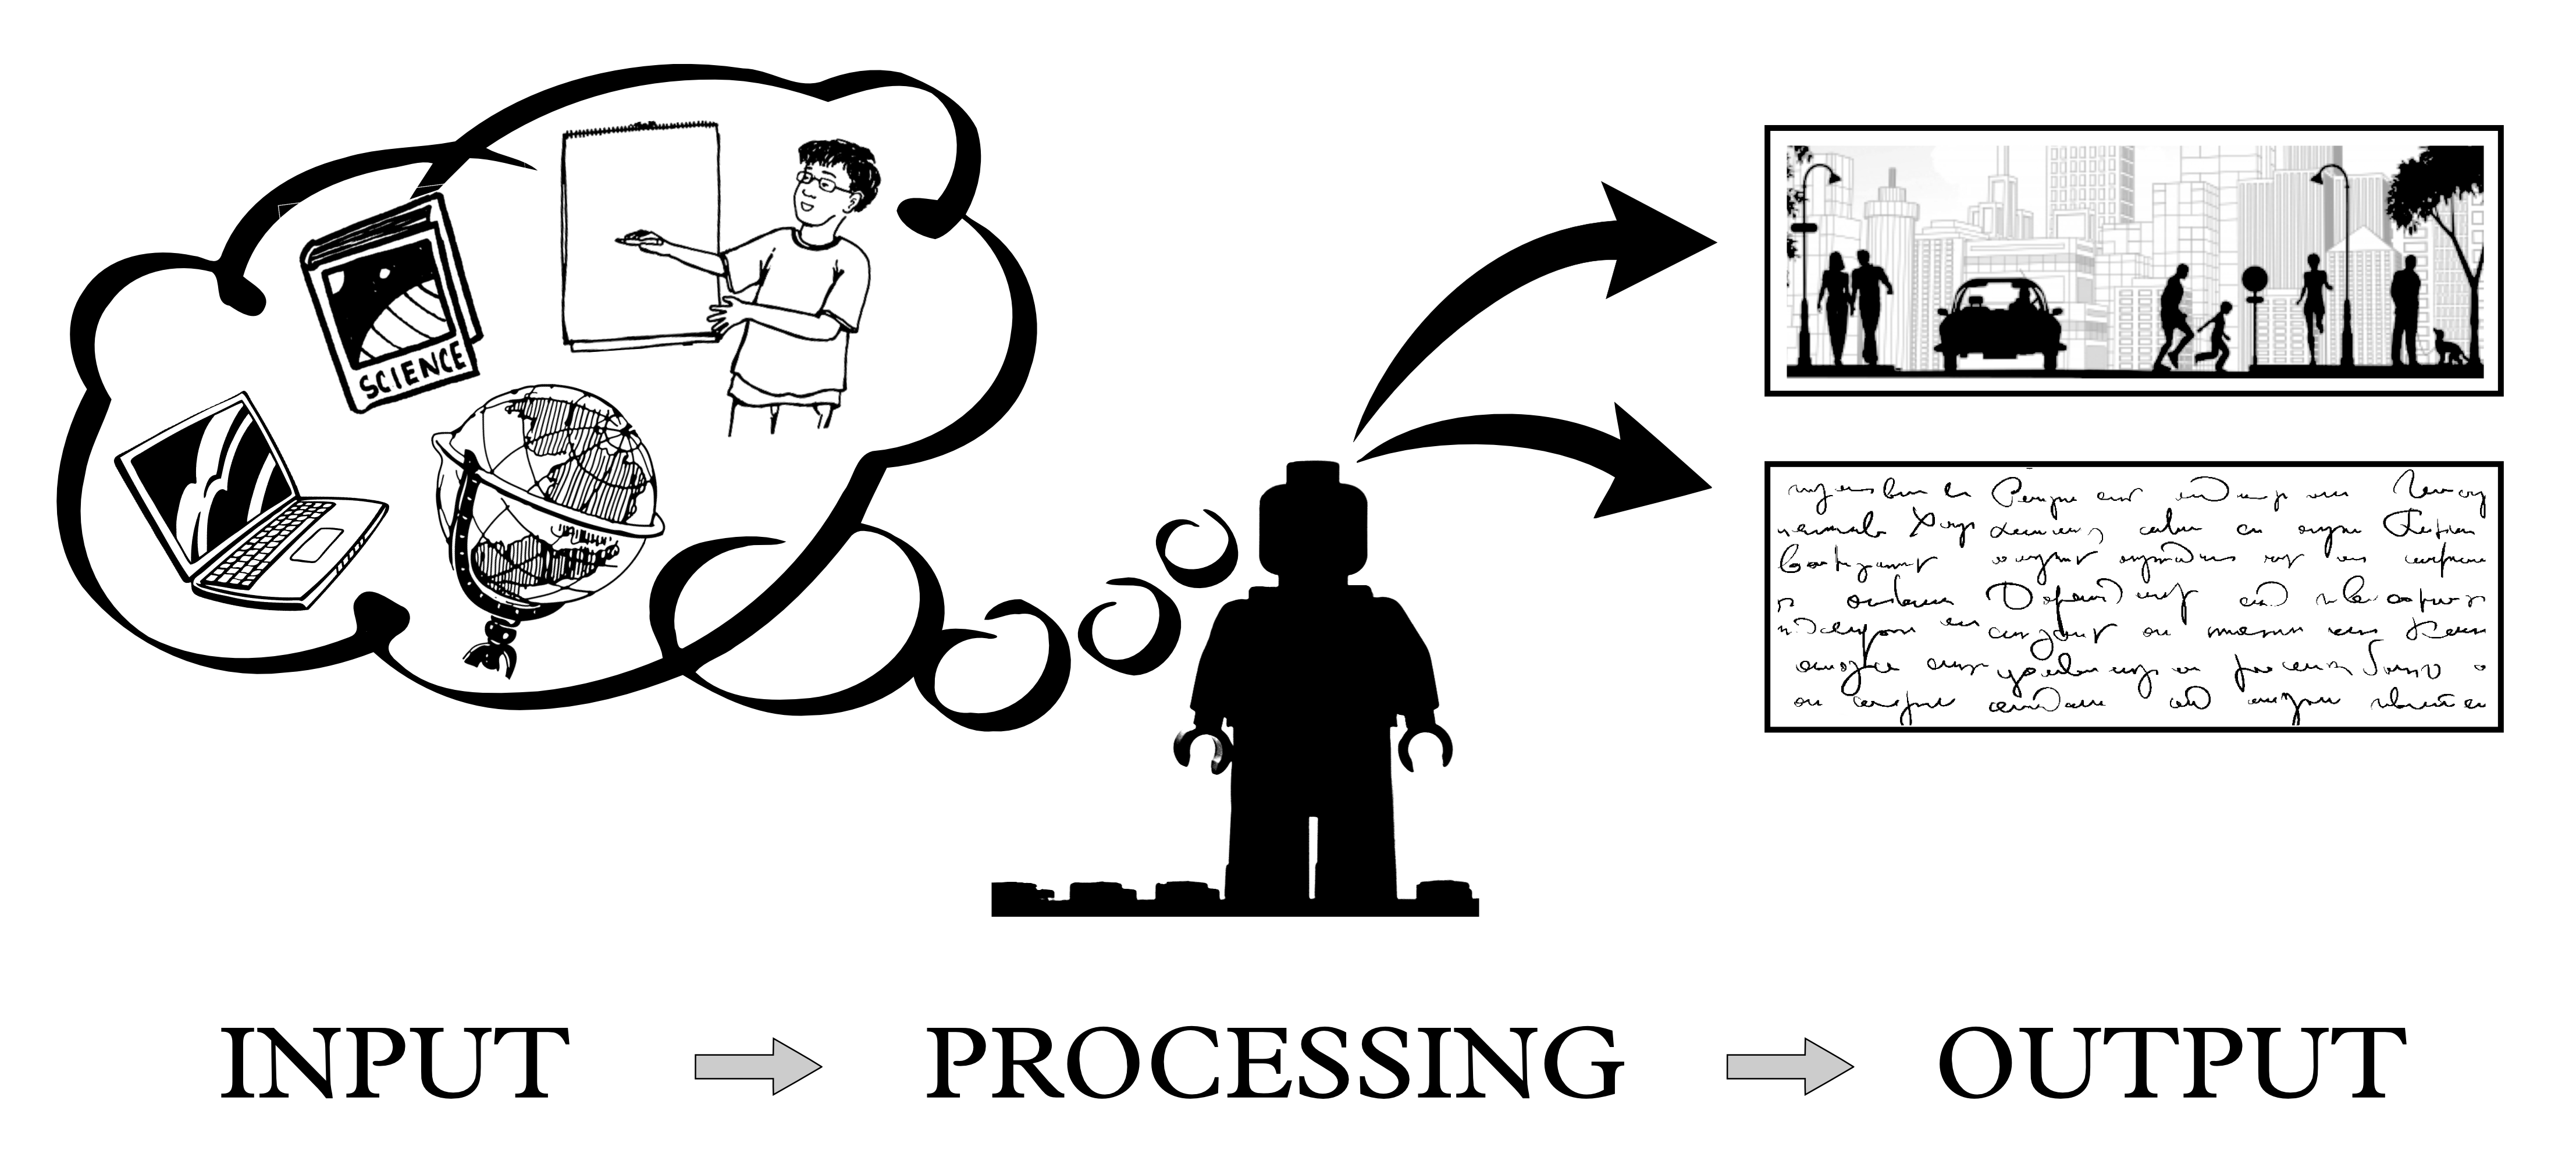
\includegraphics[width=\textwidth]{../../../img/innersim.png}

When you move to catch a falling pen, or notice that your friend is upset just by the way they entered the room, you're using your \textbf{inner simulator}.
\begin{center}
	\begin{tabular}{ | p{.5\textwidth} | p{.5\textwidth} | }
		\hline
		\textbf{Inner Simulator} & \textbf{Explicit/Verbal Models} \\ \hline
		Intuitive; part of System 1 & Analytical; part of System 2 \\ \hline
		Outputs feelings, urges, reflexes, and vivid predictions (sometimes called ``anticipations'') & Outputs arguments, calculations, and explicit models (sometimes called ``professions'') \\ \hline
		Learns well from experience and examples and responds to being \emph{shown} & Learns well from textbooks, statistics, Wikipedia, etc. and responds to being \emph{told} \\ \hline
		Good at social judgment, routine tasks, and any situation where you have lots of experience & Good at comparisons and reframings (e.g. noticing that \$1/day $\approx$ \$350/year) \\ \hline
		Powerful generator of narratives and explanations, but vulnerable to framing and subconscious question substitution & Powerful generator of plans and models, but vulnerable to distortion from wishful thinking and ideology \\ \hline
	 \end{tabular}
 \end{center}

\setlength{\parindent}{1.5em}
Each of us carries around a rich, complex model of the universe in our head, assembled from a lifetime of experiences and memories.  We don't have to \emph{think} about how to catch a falling pen, because our inner simulator \emph{knows} how falling objects move.  Similarly, it knows what facial expressions mean, what it's like to drive from home to work, and what sorts of things \emph{tend to go wrong} given a set of circumstances.  It's a powerful tool, and learning how to access it and when to trust it is one of the first steps to becoming a whole-brain thinker.

\section*{Prompts for your inner sim}
\setlength{\parindent}{0em}
Not every problem is appropriately addressed with your inner sim---you can imagine it as a single piece of hardware with a few built-in functions.  It's very, very good at doing those functions, and not so great with most other things (for instance, inner sim is terrible at understanding large numbers, and causes us to donate \emph{the same amount of money} to save 8,000 or 800,000 hypothetical birds from oil spills).  Here are three types of question your inner sim \emph{is} good at answering:

\subsubsection{What happens next?}
Start a ``mental movie'' by concretely visualizing a situation, and see what your brain \emph{expects to happen.}  Given the following inputs, what would be the output?
\begin{itemize}
	\item \textbf{Input:} A laptop is balanced half-off, half-on the edge of a table in a crowded, busy office.
	\item \textbf{Input:} You lift a piece of watermelon to your mouth and take a bite.
	\item \textbf{Input:} You sneak up on a friend at work, take aim with your water gun, and pull the trigger.
\end{itemize}

\subsubsection{How shocked am I?}
Check your ``surprise-o-meter''---visualize a scenario from start to finish, and see whether you ``buy'' that things would actually play out that way.
\begin{itemize}
	\item \textbf{Input:} You've purchased food for a 25-person party, and 20 people show up.
	\item \textbf{Input:} Same party, but \emph{70} people show up.
	\item \textbf{Input:} You finish your current project in less than half the time you allotted for it.
\end{itemize}

\subsubsection{What went right/wrong?}
Use your ``pre-hindsight''---start by assuming that your current plan has utterly failed (or gone extremely well, but that's the side we're already biased toward believing).  What explanation leaps to mind about why this happened?
\begin{itemize}
	\item \textbf{Input:} Think of a \emph{specific} email you intend to send in the next few days.  Turns out, the person you sent it to was extremely irritated by it.
	\item \textbf{Input:} Imagine you receive a message from yourself from the future, telling you that you should \emph{absolutely} stay at your current job, and keep up the good work.
	\item \textbf{Input:} It's now been three months since your CFAR workshop, and you have yet to make deliberate use of your inner simulator.
\end{itemize}
\clearpage

\section*{Being specific: Making good use of your inner simulator}
Like most algorithms, your inner simulator will output good and useful information if you give it good and useful input, and it will output useless garbage if that's what you feed it.  It's an especially good check on wishful thinking and motivated cognition---just imagine its response to a list of New Year's resolutions---but you need to make sure that you aren't rigging the game by phrasing questions the wrong way.

\setlength{\parindent}{1.5em}
Two useful strategies for avoiding vague, open-ended ``garbage'' are sticking to \emph{concrete examples} and looking for \emph{next actions}.

\subsubsection{Asking for Examples}
\newenvironment{blockquote}{%
  \par%
  \medskip
  \leftskip=4em\rightskip=2em%
  \noindent\ignorespaces}{%
  \par\medskip}
\begin{blockquote}
``It's just so \emph{frustrating.}  It's like, every little thing turns into a fight, you know?  And then it's \emph{my} fault that we're fighting, and I have to either pick between defending myself or smoothing things over, and since I'm the only one who ever wants to smooth things over, that means that I'm always the one apologizing.  And last week---I told you about what happened while we were stuck in traffic, right?  No?  So, like, out of \emph{nowhere,} while I'm trying to focus on not getting into a wreck, all of a sudden we're back talking about grad school \emph{again}\ldots''
\end{blockquote}

In a situation like this, your inner sim has nothing to grab onto---everything is vague, everything is open to interpretation, and clich\'es and stereotypes are filling in for actual understanding.  It could be that your friend is in the right, and needs your commiseration; it could be that the situation calls for some harsh truths and tough love.  How can you tell, one way or another?  Try some of these:
\begin{itemize}
	\item{What were the last couple of things you fought about?}
	\item{What were you talking about right before grad school came up?}
	\item{When you say you're the only one who wants to smooth things over, what do you mean?  What are you seeing and hearing that give you that sense?}
\end{itemize}

When it's just ``every little thing turns into a fight,'' your inner sim literally doesn't know what to think---there are too many possibilities.  But when the argument started with ``Do we really have to go over to Frank's \emph{again?}'' or with ``Oh, hey, I see you got new shoes.  Nice!'' you have a much better clearer sense of what the situation really looks like.

Asking for examples is a handy technique for any conversation.  When you keep your inner simulator engaged, and keep feeding it data, you might notice that it's easier to:


So, those are three common and useful function calls, but don't forget---the algorithm is only as good as the input it is given.  Your inner simulator is especially good at being a check on wishful thinking or what you feel like you \emph{ought} to believe---picture its response to a list of New Year's Resolutions---but you need to make sure that your explicit/verbal models aren't rigging the game by phrasing questions the wrong way.  If you pass your inner simulator vague, open-ended input, it will happily give you 
























Being Specific: Making the Best Use of Your Inner Simulator 

These are three ways you can make function calls on your Inner Simulator, but how can you make sure you?re passing it the best inputs?  Your Inner Simulator is especially good at being a check on wishful thinking or what you feel like you ought to believe, but you need to make sure your explicit/verbal models aren?t rigging the game by phrasing questions the wrong way.  

By being specific, concrete, and vivid, you can mostly avoid getting stuck in Garbage In, Garbage Out.  Using concrete examples and next actions will help.

Ask for Examples!
For a concrete example of using examples, try this story from Surely You?re Joking, Mr. Feynman!
I had a scheme, which I still use today when somebody is explaining something that I'm trying to understand: I keep making up examples. For instance, the mathematicians would come in with a terrific theorem, and they're all excited. As they're telling me the conditions of the theorem, I construct something which fits all the conditions. You know, you have a set (one ball) - disjoint (two balls). Then the balls turn colors, grow hairs, or whatever, in my head as they put more conditions on. Finally they state the theorem, which is some dumb thing about the ball which isn't true for my hairy green ball thing, so I say, "False!"
If it's true, they get all excited, and I let them go on for a while.  Then I point out my counterexample.  
"Oh.  We forgot to tell you that it's Class 2 Hausdorff homomorphic."
Your inner simulator needs something to visualize.  Just saying something as words isn?t enough.  You want something specific that your imagination can interact with.  You can ask yourself for examples, too!

Asking for examples is a really handy thing to do in conversation.  When you keep your Inner Simulator engaged during a conversation, and keep feeding it data, you might notice that it?s easier to:
1. Notice if your friend?s claim is false ? Just like Feynman, you may be able to notice where the error is, instead of just having a vague sense of something not adding up if you?re concrete.
2. Notice if you?re misunderstanding your friend ? When we listen to someone else, we try to approximate and anticipate what they?re explaining.  If you ask for examples from your friend, you can see if you?ve been accidentally adding or leaving out extraneous features on yours.
3. Notice if you?re the one who?s wrong ? It?s easy to avoid noticing if you?ve made a mistake; it?s painful!  The more concrete your disagreement is, the easier it is to notice if there?s a flaw in your own argument and to own up to it.

Next Actions

A goal isn?t the same thing as a plan.  I might have the goal of exercising more, but to have a plan I need to think about when I?ll go to the gym, what I?ll do, and how I?ll remember in the moment.  

But before I get up to any of those parts of the plan, I?ll need to take my next action, which might be printing out my gym coupon or setting a reminder in my calendar or choosing a time to go buy workout clothes.  A next action is the step that sets your plan in motion.  It?s the first thing you?d have to do to keep the plan going, which is often as pedestrian as putting something on your calendar or placing a library hold or asking someone to have coffee to talk over the plan.  Often, when you?re deciding on a next action, it?s helpful to think about a trigger ? some specific event or time that reminds you to do your next action (such as 5pm Tuesday, or when my boss returns my email, or when I wake up tomorrow morning )

Write down one goal you have (a larger scale thing you want to accomplish):
Take a few minutes to think about your plan to make this goal happen.  What?s the next action you need to take to get the plan moving?
What specific trigger will let you know when it?s time to complete this next action?
Now practice going through this process a few more times: 
Goal:
Next action: 
Trigger: 
Goal: 
Next action: 
Trigger:
Inner Simulator Practice: Murphyjitsu!

Murphy?s Law says that anything that can go wrong will go wrong, but you can use some of the skills and safeguards you?ve learned for your Inner Simulator to anticipate and evade these hazards.
Step 1: Pick a plan/project/goal
Step 2: Make it specific enough to visualize. 
What?s the next action you would need to take to keep this project/plan moving forward?  It should be concrete enough that you can picture yourself doing it, not something vague like ?work out more.?
Step 3: Check your surprise-o-meter
Visualize putting this plan in motion, then ask, how surprised would I be if this plan failed?  If you?d be shocked, then you?re done!  Otherwise, continue to step 4.
Step 4: Use Pre-Hindsight
Your plan didn?t work!  And it failed at the stage of the next action you wrote in Step 2!  What happened?
Step 5: Use Looking Forward
What action would you have had to take to prevent this particular failure mode?  Visualize taking this preemptive action and then ask ?What comes next??  Have you successfully defused the danger?  Did you create a new weak point to patch?
Step 6: Iterate!
Repeat Steps 3-5 several times (sometimes this technique is called ?Simulate 17 times, act once?).  What else might have gone wrong?  What could have prevented it?  You?re battle-hardening your plan against happenstance and poor habits.  Remember that this should be very quick ? all ?17? iterations should take maybe a few minutes total.

\end{document}